\chapter{Desarrollo}
\label{desarrollo}

En este capítulo se detalla el proceso de recolección de las mamografías y se
presenta el método de preprocesamiento propuesto.

\section{Etapa de recolección}

Las mastografías fueron recolectadas en el Hospital de Alta Especialidad Juan
Graham Casasús. Los casos originalmente son almacenadas en discos compactos y
organizados con un archivo DICOMDIR. 

\begin{table}[h]
  \caption[Etiquetas DICOM]{Etiquetas DICOM que permanecen en la imagen} 
  \label{table:dicomtags}
\begin{center}
{\scriptsize
    \begin{tabular}{c|c}
    \hline

    {\bf Etiquetas} & 
    {\bf Descripción} \\
    \hline
        (7fe0, 0010) & Datos de pixel\\
        (0028, 0103) & Representación de píxeles \\
        (0028, 0010) & Filas \\
        (0028, 0011) & Columnas \\
        (0028, 0100) & Bits alojados \\
        (0028, 0101) & Bits almacenados \\
    \hline
    \end{tabular}
}
\end{center}
\end{table}

Para extraer las imágenes y organizarlas, se utilizó un \textit{script}
programado con el lenguaje de programación Python~\cite{python} y la librería
PyDICOM~\cite{pydicom}. Se removieron las etiquetas que almacenan los datos
privados de los pacientes y los etiquetas que permanecen en las imágenes se
pueden ver en la Tabla \ref{table:dicomtags}.

\section{Método propuesto}

Cada mamograma recolectado fue procesado con un método híbrido de cinco etapas.
En la Figura \ref{fig:flowchart} se presenta un diagrama de flujo con las
etapas del método híbrido. Utilizamos el lenguaje de programación
Matlab~\cite{matlab} más la utilidad de procesamiento de imágenes Image
Processing Toolbox~\cite{ipt}.

\shorthandoff{>} % hack to combine tikZ and Spanish
    
% -------------------------------------------------
% Set up a new layer for the debugging marks, and make sure it is on
% top

\pgfdeclarelayer{marx}
\pgfsetlayers{main,marx}
% A macro for marking coordinates (specific to the coordinate naming
% scheme used here). Swap the following 2 definitions to deactivate
% marks.
\providecommand{\cmark}[2][]{%
  \begin{pgfonlayer}{marx}
    \node [nmark] at (c#2#1) {#2};
  \end{pgfonlayer}{marx}
  } 
\providecommand{\cmark}[2][]{\relax} 
% -------------------------------------------------
\begin{figure}[h]
\begin{center}
\begin{tikzpicture}[%
    >=triangle 60,              % Nice arrows; your taste may be different
    start chain=going below,    % General flow is top-to-bottom
    node distance=6mm and 60mm, % Global setup of box spacing
    every join/.style={norm},   % Default linetype for connecting boxes
    ]

{\small\ttfamily\fontfamily{lmodern}\selectfont
% ------------------------------------------------- 
% A few box styles 
% <on chain> *and* <on grid> reduce the need for manual relative
% positioning of nodes
\tikzset{
  base/.style={draw, on chain, on grid, align=center, minimum height=4ex},
  proc/.style={base, rectangle, text width=8em},
  test/.style={base, diamond, aspect=2, text width=5em},
  term/.style={proc, rounded corners},
  % coord node style is used for placing corners of connecting lines
  coord/.style={coordinate, on chain, on grid, node distance=6mm and 25mm},
  % nmark node style is used for coordinate debugging marks
  nmark/.style={draw, cyan, circle, font={\sffamily\bfseries}},
  % -------------------------------------------------
  % Connector line styles for different parts of the diagram
  norm/.style={->, draw, blue},
  free/.style={->, draw, green},
  cong/.style={->, draw, red},
  it/.style={font={\small\itshape}}
}
% -------------------------------------------------
% Start by placing the nodes
% Use join to connect a node to the previous one a

\node [term, it] (p0) {Start};
\node [proc, fill=violet!30, join] (p1) {Reduction of work area};
\node [test, join] (t1) {12 bits image?};
% No join for exits from test nodes - connections have more complex
% requirements
% We continue until all the blocks are positioned
\node [proc, fill=brown!30] (p2) {Conversion to 16 bits};
\node [proc, fill=blue!30, join] (p3) {Adaptive Median Filter};
\node [proc, fill=green!30, join] (p4) {Histogram Equalization};
\node [proc, fill=red!30, join] (p5) {Image shrinking};
\node [term, join, it]      {End};
% We position the next block explicitly as the first block in the
% second column.  The chain 'comes along with us'. The distance
% between columns has already been defined, so we don't need to
% specify it.

% -------------------------------------------------
% Now we place the coordinate nodes for the connectors with angles, or
% with annotations. We also mark them for debugging.

\node [coord, left=of t1]  (c1)  {}; %\cmark{1}   
 
% -------------------------------------------------
% A couple of boxes have annotations

% -------------------------------------------------
% All the other connections come out of tests and need annotating
% First, the straight north-south connections. In each case, we first
% draw a path with a (consistently positioned) annotation node, then
% we draw the arrow itself.
\path (t1.south) to node [near start, xshift=1em] {$yes$} (p2);
  \draw [->,blue] (t1.south) -- (p2);

% -------------------------------------------------
% Finally, the twisty connectors. Again, we place the annotation
% first, then draw the connector
\path (t1.west) to node [near start, yshift=-1em] {$no$} (c1); 
  \draw [->,blue] (t1.west) -- (c1) |- (p2);

% -------------------------------------------------

    \draw[brown, thick] ($(p3.north west)+(-0.3,0.3)$)  rectangle ($(p5.south east)+(0.3,-0.3)$) 
    node [right]{label};
}
\end{tikzpicture}
\end{center}
  \caption{Preprocessing method applied to each image in the collection} 
  \label{fig:flowchart} 
\end{figure}

\shorthandon{>} 

\subsection{Reducción del área de trabajo}

La primera etapa del método consiste en eliminar la región oscura que cubre
gran parte de la imagen para acelerar el tiempo de ejecución de los
procedimientos posteriores. El enfoque es similar al expuesto por Dehghani y
Holguín \cite{dehghani2011method, holguinpre}.

% thresholding
Aplicamos un método de tres fases para lograr la reducción: umbralización,
eliminación de objetos y corte automático. En la Figura \ref{reduction} se
muestra cada una de estas fases. 

La primera fase es la \textit{umbralización}, cuyo propósito es separar el
objeto de interés del fondo. Para lograr este cometido, inicialmente la imagen
es convertida de simple precisión a doble precisión, lo que nos permite obtener
mejores resultados en el proceso de binarización. Después, se calcula el valor
\textit{umbral} de la imagen con la función \texttt{graytresh} de Matlab, esta
función implementa el método de Otsu \cite{otsumethod}. El valor umbral que se
obtiene como resultado es usado para clasificar los pixeles como 0 ó 1. El
tercer paso es la binarización, que es ejecutada utilizando una función la
función \texttt{im2bw} de Matlab. El resultado se muestra en la Figura
\ref{area:b}.

\begin{figure}[h]
    \centering

    \subfloat[Imagen original\label{area:a}]{\includegraphics[height=35mm]{images/area/original.jpg}}
    \subfloat[Binarización\label{area:b}]{\includegraphics[height=35mm]{images/area/whiteandblack.jpg}}
    \subfloat[No etiquetas\label{area:c}]{\includegraphics[height=35mm]{images/area/deleteobj.jpg}}

    \bigskip
    
    \subfloat[Dibujo de bordes\label{area:d}]{\includegraphics[height=35mm]{images/area/bordering.jpg}}
    \subfloat[Imagen reducida\label{area:e}]{\includegraphics[height=35mm]{images/area/reduced.jpg}}

  \caption[Reducción del área de trabajo]
  {Reducción del área de trabajo.}
  \label{reduction}
\end{figure}

La segunda fase es \textit{eliminación de objetos} que consiste en remover
todos los objetos de la imagen a excepción del área de interés. Por ejemplo, en
la Figura \ref{area:b} podemos ver una etiqueta en la esquina superior derecha
que fue removida en la Figura \ref{area:c}. Lo que realmente hacemos es remover
todos los objetos con menos de 10'000 píxeles, ya que consideramos que un seno
jamás será menor de 10'000 píxeles. Este procedimiento es ejecutado utilizando
la función Matlab llamada \texttt{bwareaopen}.

Finalmente, la fase de corte automático se divide en dos pasos. El primero es
determinar la localización del borde de la imagen, lo que es logrado con la
función de Matlab llamada \texttt{bwboundaries}. Esta función encuentra los
bordes de un objeto utilizando el algoritmo Moore-Neighbor modificado por el
criterio de paro de Jacob \cite{gonzalez2009digital}. Los bordes son utilizados
para determinar los puntos extremos de cada seno (ver \ref{area:d}). El segundo
paso es hacer el corte usando estos puntos extremos (ver \ref{area:e}). 

\subsection{Conversión de bits}

Como ya se mencionó antes, las imágenes están en el formato DICOM. El formato
DICOM representa las imágenes con 4'096 niveles de grises, esto es 12 bits de
profundidad. Matlab representa estas imágenes utilizando 16 bits de
profundidad, o sea, 65'536 niveles de grises \cite{mustra2008efficient}. Cuando
una imagen de 12 bits es visualizada con un visor de 16 bits, esta luce oscura,
ver Figura \ref{bits}. Para mostrar la imagen correctamente esta necesita ser
convertida a una imagen de 16 bits. Se aplicó la Ecuación \ref{eq:bitconv} a
cada pixel en la imagen para realizar la conversión.

\begin{equation}
\label{eq:bitconv}
    \begin{split}
            \ell &= \frac{2^{n}}{2^{m}} \\
            c_{x,y} &= i_{x, y} \times \ell,
    \end{split}
\end{equation}

\noindent donde $\ell$ es un valor escalar, $n$ es el número de bits de la imagen
objetivo, $m$ es el número de bits en la imagen original. La vieja matriz es
representada con $i$ y la nueva con $c$. El par $x$ y $y$ representan la
posición de los píxeles en cada matriz.

% case number 16, rcc
\begin{figure}[h]
    \centering

    \subfloat[12 bits\label{bits:a}]{\includegraphics[height=55mm]{images/bits/12bits.jpg}}
    \subfloat[16 bits\label{bits:b}]{\includegraphics[height=55mm]{images/bits/16bits.jpg}}

  \caption[Conversión de bits]
  {Conversion de bits}
  \label{bits}
\end{figure}

\subsection{Eliminación de ruido}

En este trabajo nos enfocamos en remover el ruido impulsivo (también llamado
ruido sal y pimienta) debido a que es un procedimiento relativamente simple. El
filtro de la mediana es muy común para remover el ruido impulsivo, sin embargo,
también \textit{suaviza} la imagen de tal forma que se pierde información sobre
algunas lesiones milimétricas como las microcalcificaciones. Versiones
mejoradas del filtro de la mediana han sido desarrolladas para corregir estas
deficiencias.

\shorthandoff{>} % hack to combine tikZ and Spanish
    \pgfdeclarelayer{myback}
    \pgfsetlayers{myback,background,main}

\begin{figure}[h]
\centering

\subfloat[Ni $Zmed$ ni $Zxy$ son ruido\label{fig:nochanges}]{
    \begin{tikzpicture}

    \tikzset{myfillcolor/.style = {draw, fill=#1}}%
    \NewDocumentCommand{\fhighlight}{O{blue!25} m m}{%
        \draw[myfillcolor=#1] (#2.north west) rectangle (#3.south east);
    }
        \draw[xstep=0.80cm, ystep=0.80, color=blue] (0,0) grid (4,4);
        \matrix (m) [matrix of nodes,
        inner sep=0pt,
        anchor=south west,
        font=\sffamily\small,
        ampersand replacement=\&,
        nodes={inner sep=0pt, text width=0.80cm, align=center, minimum height=0.80cm}
        ]{
        159 \& 234 \& 210         \& 131 \& 120 \\
        392 \& 100 \& 91          \& 120 \& 138 \\
        205 \& 104 \& \textbf{107}\& 115 \& 233 \\
        332 \& 94  \& 96          \& 117 \& 420 \\
        39  \& 304 \& 349         \& 300 \& 130 \\
        };

    \begin{pgfonlayer}{myback}
    \fhighlight{m-2-2}{m-4-4}
    \fhighlight[green!40]{m-3-3}{m-3-3}
    \fhighlight[red!40]{m-3-2}{m-3-2}
    \end{pgfonlayer}

    \end{tikzpicture}
}
\hspace{12pt}
\subfloat[$Zxy$ es ruido\label{fig:zxynoise}]{
    \begin{tikzpicture} 

    \tikzset{myfillcolor/.style = {draw, fill=#1}}%
    \NewDocumentCommand{\fhighlight}{O{blue!25} m m}{%
        \draw[myfillcolor=#1] (#2.north west) rectangle (#3.south east);
    }

        \draw[xstep=0.80cm, ystep=0.80, color=blue] (0,0) grid (4,4);
        \matrix[matrix of nodes,
        inner sep=0pt,
        anchor=south west,
        font=\sffamily\small,
        ampersand replacement=\&,
        nodes={inner sep=0pt, text width=0.80cm, align=center, minimum height=0.80cm}
        ]{
        159 \& 234 \& 210         \& 131 \& 120 \\
        392 \& 99  \& 91          \& 135 \& 138 \\
        205 \& 109 \& \textbf{82} \& 117 \& 233 \\
        332 \& 90  \& 95          \& 149 \& 420 \\
        39  \& 304 \& 349         \& 300 \& 130 \\
        };

    \begin{pgfonlayer}{myback}
    \fhighlight{m-2-2}{m-4-4}
    \fhighlight[green!40]{m-3-3}{m-3-3}
    \fhighlight[red!40]{m-2-2}{m-2-2}
    \end{pgfonlayer}

    \end{tikzpicture}
}

% space
\subfloat[$Zmed$ es ruido\label{fig:zmednoise}]{
    \begin{tikzpicture}

    \tikzset{myfillcolor/.style = {draw, fill=#1}}%
    \NewDocumentCommand{\fhighlight}{O{blue!25} m m}{%
        \draw[myfillcolor=#1] (#2.north west) rectangle (#3.south east);
    }

        \draw[xstep=0.80cm, ystep=0.80, color=blue] (0,0) grid (4,4);
        \matrix[matrix of nodes,
        inner sep=0pt,
        anchor=south west,
        font=\sffamily\small,
        ampersand replacement=\&,
        nodes={inner sep=0pt, text width=0.80cm, align=center, minimum height=0.80cm}
        ]{
        159 \& 234 \& 110        \& 131 \& 120 \\
        192 \& 230 \& 230        \& 135 \& 138 \\
        105 \& 230 \& \textbf{3} \& 230 \& 233 \\
        132 \& 90  \& 230        \& 149 \& 220 \\
        139 \& 104 \& 149        \& 100 \& 130 \\
        };

    \begin{pgfonlayer}{myback}
    \fhighlight{m-2-2}{m-4-4}
    \fhighlight[green!40]{m-3-3}{m-3-3}
    \fhighlight[red!40]{m-2-2}{m-2-3}
    \fhighlight[red!40]{m-3-2}{m-3-2}
    \fhighlight[red!40]{m-3-2}{m-3-2}
    \fhighlight[red!40]{m-4-3}{m-4-3}
    \fhighlight[red!40]{m-3-4}{m-3-4}
    \end{pgfonlayer}

    \end{tikzpicture}
}
\hspace{12pt}
\subfloat[Incrementa el tamaño de $w$\label{fig:repeat}]{
    \begin{tikzpicture} 

    \tikzset{myfillcolor/.style = {draw, fill=#1}}%
    \NewDocumentCommand{\fhighlight}{O{blue!25} m m}{%
        \draw[myfillcolor=#1] (#2.north west) rectangle (#3.south east);
    }

        \draw[xstep=0.80cm, ystep=0.80, color=blue] (0,0) grid (4,4);
        \matrix[matrix of nodes,
        inner sep=0pt,
        anchor=south west,
        font=\sffamily\small,
        ampersand replacement=\&,
        nodes={inner sep=0pt, text width=0.80cm, align=center, minimum height=0.80cm}
        ]{
        159 \& 234 \& 110        \& 131 \& 120 \\
        192 \& 230 \& 230        \& 135 \& 138 \\
        105 \& 230 \& \textbf{3} \& 230 \& 233 \\
        132 \& 90  \& 230        \& 149 \& 220 \\
        139 \& 104 \& 149        \& 100 \& 130 \\
        };

    \begin{pgfonlayer}{myback}
    \fhighlight{m-1-1}{m-5-5}
    \fhighlight[green!40]{m-3-3}{m-3-3}
    \fhighlight[red!40]{m-5-1}{m-5-1}
    \end{pgfonlayer}

    \end{tikzpicture}
}
\caption[Funcionamiento del algoritmo AMF]{Funcionamiento del algoritmo AMF en diversos escenarios.}
\label{fig:amf} 
\end{figure}


\shorthandon{>} 

Utilizamos el Filtro Adaptativo de la Mediana (AMF\footnote{Adaptive Median
Filter}) tal como es implementado por González~\cite{gonzalez2009digital}. La
idea principal de AMF es remover los \textit{píxeles ruidosos}, que son
aquellos rodeados por píxeles vecinos con valores muy diferentes. Tan pronto
como AMF detecta un pixel ruidoso lo reemplaza por el valor de la mediana de
los píxeles vecinos.

El algoritmo usa una ventana $w$ con un tamaño de $3\times3$ que recorre toda
la imagen. En cada ubicación, el valor mínimo $Zmin$, el valor máximo $Zmax$ y
la mediana $Zmed$ son calculados. $Zxy$ es el centro de $w$. $Smax$ es el tamaño
máximo que $w$ puede alcanzar.

% pseudocode
% ref this code
\algrenewcommand{\alglinenumber}[1]{\footnotesize\textbf{\ttfamily#1}} 
% avoid two points in the numbering and add ttfamily font
\algrenewcommand\algorithmicif{\ttfamily\textbf{{if}}}
\begin{algorithm}
\caption{AMF implementado por \cite{gonzalez2009digital}}
\begin{algorithmic}[1]
% initialize variables ?
\State Level A:
\If {$Zmin < Zmed < Zmax$}
        \State go to Level B
\Else
    \State increase the window size % or w = w + 2
    \If {$w \leq S_{max}$}
       \State repeat Level A 
    \Else
        \State output is $Zmed$
    \EndIf
\EndIf
\State Level B:
\If {$Zmin < Zxy < Zmax$}
    \State output is $Zxy$
\Else
    \State output is $Zmed$
\EndIf
\end{algorithmic}
\end{algorithm}

AMF trabaja en dos niveles, nivel A y nivel B. En el nivel A (línea 2) se
identifica $Zmed$ como impulso cuando la condición es falsa. En este caso, el
tamaño de $w$ incrementa (línea 5) y el nivel A es repetido mientras $w$ es
menor o igual a su tamaño máximo $Smax$ (línea 6); de otra forma, el pixel
central toma el valor de $Zmed$ que es la mediana de los píxeles en la ventana
$w$ (línea 9).

Si la condición en la línea 2 es verdadera se descarta $Zmed$ como impulso y el
algoritmo continua en el nivel B. En el nivel B, cuando la condición en la
línea 11 es verdadera, entonces $Zxy$ no es un impulso, en ese caso no hay
ningún cambio (línea 12); de otra forma, el pixel cantral toma el valor de
$Zmed$.

\subsection{Mejora del contraste}

Para mejorar el contraste aplicamos la ecualización de histogramas. Debido a la
efectividad probada del algoritmo CLAHE, como se discutió en el capítulo
anterior, utilizamos la función llamada \texttt{adaptivehisteq} de Matlab IPT
que implementa CLAHE. Los parámetros de esta función son modificados con ayuda
de los radiólogos. La configuración final es aplicada a un área específica de
la imagen. En la Figura \ref{img:clahe} se muestra un ejemplo de la mejora de
contraste utilizando CLAHE.

% show lesion images
\begin{figure}[h!]
  \begin{center}
    \subfloat[\label{contr:a}]{\includegraphics[height=35mm]{images/contrast/before-clahe}}
    \hspace{12pt}
    \subfloat[\label{contr:b}]{\includegraphics[height=35mm]{images/contrast/before-clahe-hist}}
    \\
    \subfloat[\label{contr:c}]{\includegraphics[height=35mm]{images/contrast/after-clahe}}
    \hspace{12pt}
    \subfloat[\label{contr:d}]{\includegraphics[height=35mm]{images/contrast/after-clahe-hist}}
  \end{center} 

  \caption[Ecualización de histogramas]{Close-up of a mammogram. \protect\subref{contr:a} Original lesion area,
  \protect\subref{contr:b} histogram of \protect\subref{contr:a}, \protect\subref{contr:c} same lesion
  area after CLAHE has been applied to it, \protect\subref{contr:d} histogram of
  \protect\subref{contr:c}.} 

  \label{img:clahe} 
\end{figure}

\subsection{Compresión}
\label{compression}

Como complemento en la fase final de nuestro método implementamos un algoritmo
de compresión cuyo principio radica en el \textit{encogimiento del histograma}.
La técnica utilizada fue introducida por AbuBaker~\cite{abubaker2006mammogram,
abubaker2007efficient}. El objetivo de esta técnica es comprimir una imagen
con la menor pérdida de calidad. El método aplicado tiene tres pasos:
encogimiento de la imagen, conversión de la profundidad de píxeles, y
mejoramiento de la imagen. A continuación se describen estos pasos:

\subsubsection{Encogimiento de la imagen.} 

La Figura~\ref{comp:a} es la imagen obtenida en la fase anterior y su
histograma correspondiente se puede ver en la Figura~\ref{comp:b}. De este
histograma eliminamos los niveles de grises no utilizados (o lagunas). Como
resultado obtenemos un histograma inclinado a la derecha, que se puede ver en
la Figura~\ref{comp:c}. A partir de este histograma se genera una nueva imagen
que luce muy oscura (ver Figura~\ref{comp:d}) pues los niveles de grises están
en la región derecha.

\begin{figure}[h]
  \begin{center}
    \subfloat[\label{comp:a}]{\includegraphics[height=40mm]{images/compress/original-mammogram-16bits}}
    \hspace{12pt}
    \subfloat[\label{comp:d}]{\includegraphics[height=40mm]{images/compress/dark-mammogram}}

    \bigskip

    \subfloat[\label{comp:b}]{\includegraphics[height=40mm]{images/compress/original-image-histogram}}
    \hspace{12pt}
    \subfloat[\label{comp:c}]{\includegraphics[height=40mm]{images/compress/shrunk-histogram}}
  \end{center}

  \caption[Método de encogimiento]{Método de encogimiento. En
  \protect\subref{comp:a} se visualiza la imagen de entrada,
  \protect\subref{comp:b} es el histograma de \protect\subref{comp:a},
  \protect\subref{comp:c} es el histograma  mostrado en \protect\subref{comp:b}
  después de ser encogido y \protect\subref{comp:d} es la imagen oscura
  generada a partir del histograma encogido.}
  
  \label{img:shrinking-one} 
\end{figure}

\subsubsection{Conversión de la profundidad de píxeles} 

En este paso la meta es reducir el tamaño de la imagen. Se necesitan tres
subpasos. Extraemos el histograma (ver Figura \ref{comp:e}) de la imagen
encogida, que es similar al que se muestra en Fig. \ref{comp:c}. Después, el
nivel máximo de encogimiento de la imagen es encontrado utilizando el
histograma en la Figura \ref{comp:e} calculando el porcentaje de niveles de
grises usados (valores diferentes a cero) en el array que representa el
histograma. Este porcentaje es la entrada de la función de Matlab IPT
\texttt{imadjust}. Esta función ajusta la intensidad de valores en una imagen.
Una nueva imagen de 8 bits se obtiene como resultado de esta función.

\begin{figure}[h]
  \begin{center}
    \subfloat[\label{comp:e}]{\includegraphics[height=30mm]{images/compress/dark-mammogram-histogram}}
    \hspace{12pt}
    \subfloat[\label{comp:f}]{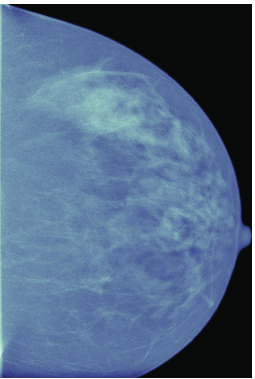
\includegraphics[height=30mm]{images/compress/compressed-mammogram-8bits}}
    \hspace{12pt}
    \subfloat[\label{comp:g}]{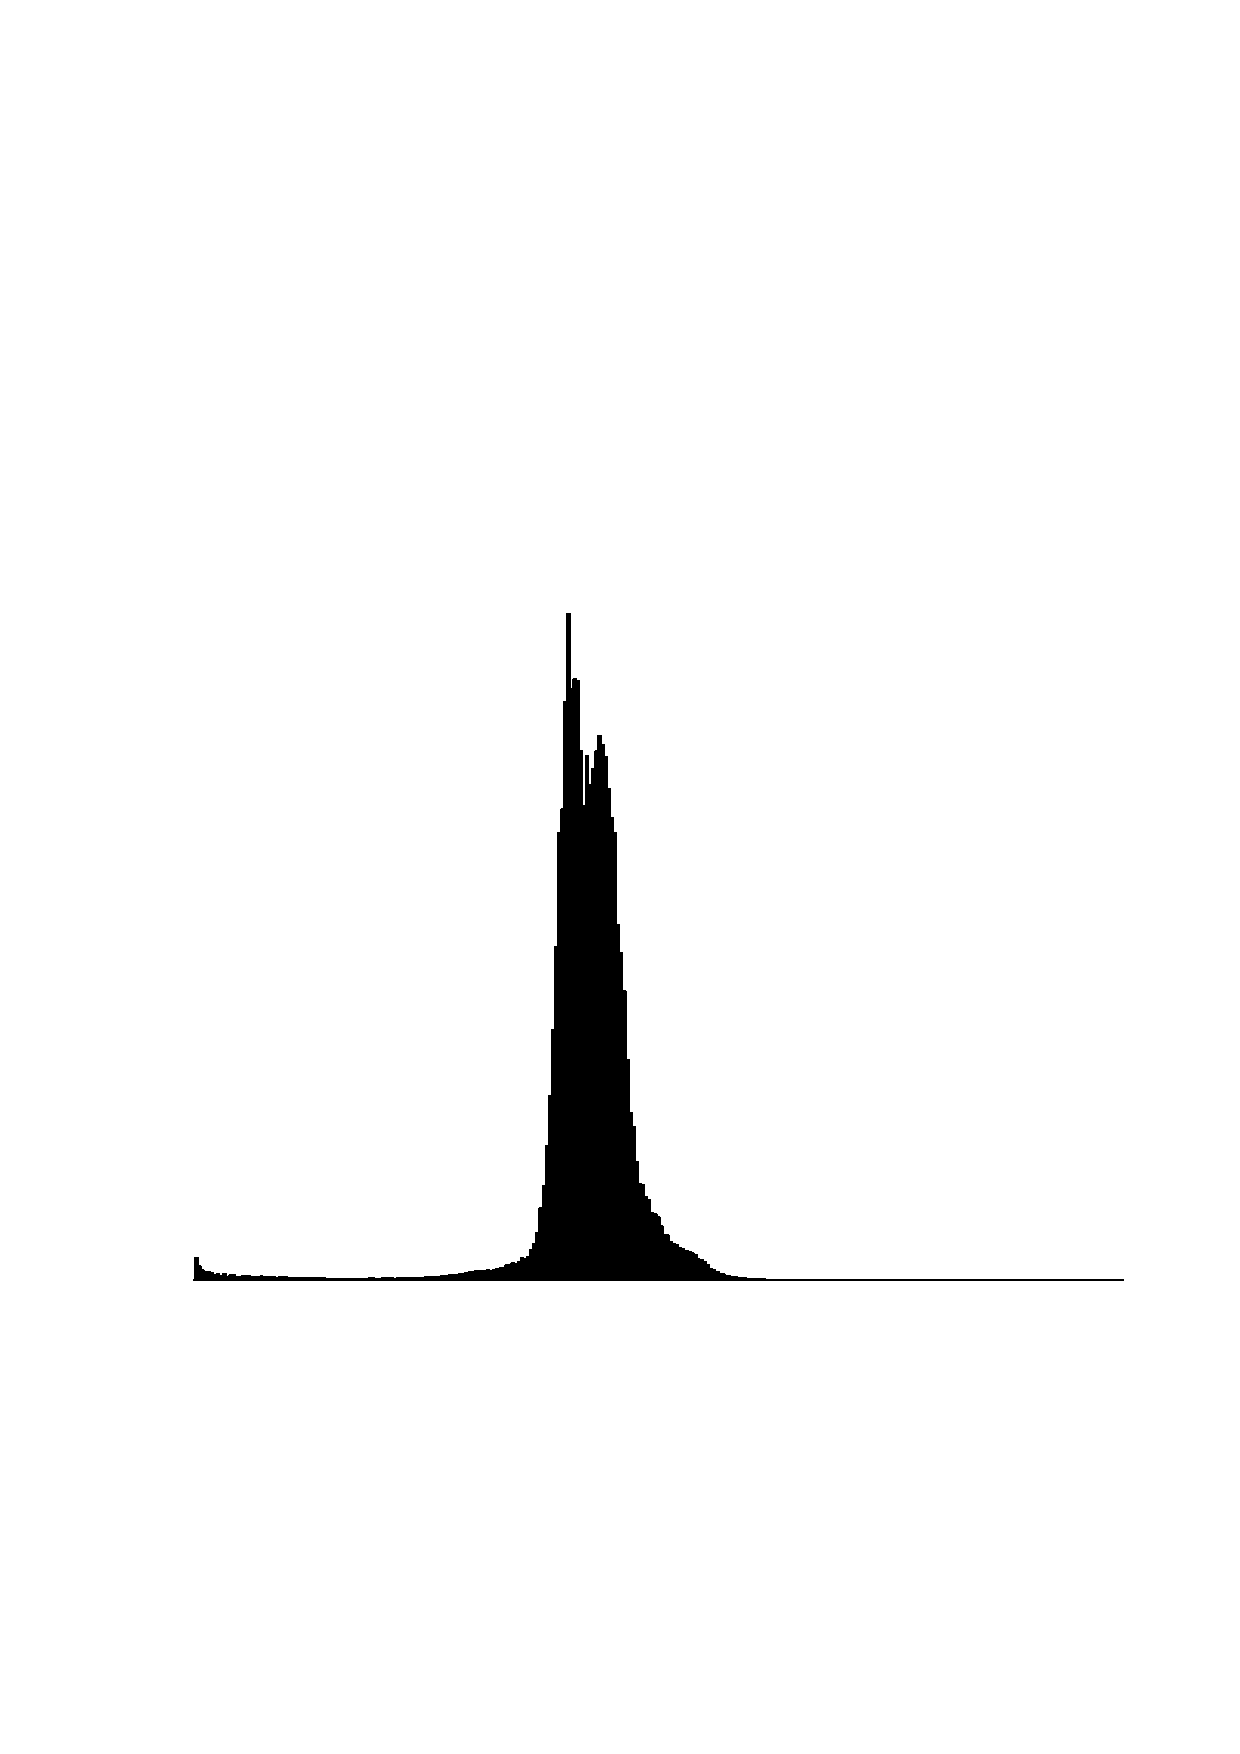
\includegraphics[height=30mm]{images/compress/compressed-mammogram-histogram}}
  \end{center}

  \caption[Compresión de la mamografía]
  {\protect\subref{comp:e} es el histograma generado a partir de la mamografía
  oscura mostrada en la Fig. \protect\ref{comp:d}, \protect\subref{comp:f} es
  la imagen de 8 bits generada a partir de \protect\subref{comp:e},
  \protect\subref{comp:g} es el histograma de la imagen
  \protect\subref{comp:f}, que es similar al histograma que se muestra en
  \ref{comp:b}}. 
  
  \label{img:shrinking-two} 
\end{figure}

El histograma mostrado en la Figura \ref{comp:b} es muy similar al histograma
de la imagen resultante mostrado en la Fig. \ref{comp:g}. Los picos son los
mismos lo que indica que la concentración de niveles de grises permanece igual.

\subsubsection{Mejora de la imagen}

El objetivo de este paso es mejorar la calidad de la imagen que se obtuvo en el 
paso anterior. 

Afterwards, image conversion from 16 to 8 bits using an efficient
coefficient takes place.

La información médica de la imagen se debe mantener. Este paso es útil como un
proceso de normalización.

\definecolor{bg}{rgb}{0.9,0.9,0.9}
\begin{minted}[linenos=true, 
               %fontfamily=fi4, 
               fontseries=ubx,
               bgcolor=bg, frame=lines]{matlab}

[height width] = size(image);
imageCopy = repmat(uint8(0), height, width);
divider = 0.0;
maxLevel = double(usedGrayLevels);

while 1
    divider = divider + 0.01;
    if maxLevel/divider <= 255
        break;
    end
end
fprintf('text');
for h=1:1:height
    for w=1:1:width
       imageCopy(h, w) = image(h, w)/divider;
    end
end
\end{minted}


